\documentclass[notheorems,mathserif,table,compress]{beamer}  %dvipdfm选项是关键,否则编译统统通不过
%%------------------------常用宏包------------------------
%%注意, beamer 会默认使用下列宏包: amsthm, graphicx, hyperref, color, xcolor, 等等
\usepackage{fontspec,xunicode,xltxtra}  % for XeTeX
\usepackage{verbatim}
\usepackage{mathabx}
\usepackage{amsfonts,amssymb}
\usepackage{iplouclistings}
%%------------------------ThemeColorFont------------------------
%% Presentation Themes
% \usetheme[<options>]{<name list>}
\usetheme{Madrid}
%% Inner Themes双精度计算
% \useinnertheme[<options>]{<name>}
%% Outer Themes
% \useoutertheme[<options>]{<name>}
\useoutertheme{miniframes} 
%% Color Themes 
%\usecolortheme[<options>]{<name list>}
%% Font Themes
\usefonttheme{serif}
\setbeamertemplate{background canvas}[vertical shading][bottom=white,top=structure.fg!7] %%背景色, 上25%的蓝, 过渡到下白.
\setbeamertemplate{theorems}[numbered]
\setbeamertemplate{navigation symbols}{}   %% 去掉页面下方默认的导航条.
\usepackage{zhfontcfg}
%\setsansfont[Mapping=tex-text]{文泉驿正黑}  %% 需要fontspec宏包
     %如果装了Adobe Acrobat,可在font.conf中配置Adobe字体的路径以使用其中文字体
     %也可直接使用系统中的中文字体如SimSun,SimHei,微软雅黑 等
     %原来beamer用的字体是sans family;注意Mapping的大小写,不能写错
     %设置字体时也可以直接用字体名,以下三种方式等同:
     %\setromanfont[BoldFont={黑体}]{宋体}
     %\setromanfont[BoldFont={SimHei}]{SimSun}
     %\setromanfont[BoldFont={"[simhei.ttf]"}]{"[simsun.ttc]"}
%%------------------------MISC------------------------
%\graphicspath{{figures/}}         %% 图片路径. 本文的图片都放在这个文件夹里了.
%%------------------------正文------------------------
\begin{document}
\XeTeXlinebreaklocale "zh"         % 表示用中文的断行
\XeTeXlinebreakskip = 0pt plus 1pt % 多一点调整的空间
%%----------------------------------------------------------
%% This is only inserted into the PDF information catalog. Can be left
%% out.
%%%
%% Delete this, if you do not want the table of contents to pop up at
%% the beginning of each subsection:
\AtBeginSection[]{                              % 在每个Section前都会加入的Frame
  \frame<handout:0>{
    \frametitle{Contents}\small
    \tableofcontents[current,currentsubsection]
  }
}

\AtBeginSubsection[]                            % 在每个子段落之前
{
  \frame<handout:0>                             % handout:0 表示只在手稿中出现
  {
    \frametitle{Contents}\small
    \tableofcontents[current,currentsubsection] % 显示在目录中加亮的当前章节
  }
}

%%----------------------------------------------------------
\title{Sovling the Possion Equation}
%\subtitle{}
\author[qiu]{主讲人~~~~~\textcolor{olive}{邱欣欣}\\
    \quad 幻灯片制作~~\textcolor{olive}{邱欣欣}}
\institute[中国海洋大学]{\small\textcolor{violet}{中国海洋大学~~信息科学与工程学院}}
\date{2014~年~3~月~28~日}
%\titlegraphic{\vspace{-6em}\includegraphics[height=7cm]{ouc}\vspace{-6em}}
\frame{ \titlepage }
%%----------------------------------------------------------
\section*{Contents}
\frame{\frametitle{}\tableofcontents}
%%----------------------------------------------------------
\section{简介}

\begin{frame}
\frametitle{Poisson Equation}
\begin{displaymath}
-\nabla^2u=f
\end{displaymath}
\begin{displaymath}
\int_{\Omega}(\nabla^2u+f)v=0
\end{displaymath}
\newline
\begin{displaymath}
\int_{\Omega}\nabla u\cdot\nabla v=\int_{\Omega}vf+\int_{\partial\Omega}vg
\end{displaymath}
\begin{displaymath}
\alpha u+\beta \frac{\partial u}{\partial n}=g \quad on \quad\partial \Omega
\end{displaymath}
\end{frame}

%
\begin{frame}
\frametitle{Galerkin finite element method}
\begin{itemize}
\item 选择$\{\phi_1,\phi_2,\cdots,\phi_n\}$为试探函数的一组基,同时定义附加函数$\phi_{n+1},\cdots,\phi_{n+n_{\partial}}$.
\begin{displaymath}
u_h=\sum_{j=1}^n u_j\phi_j+\sum_{j=n+1}^{n+n_{\partial}}u_j\phi_j
\end{displaymath}

\item $\phi_i,i=1,\cdots,n$被称作形状函数.
\end{itemize}
\end{frame}

\begin{frame}
\frametitle{Galerkin finite element method}
\begin{itemize}
\item 
\begin{displaymath}
\sum_{j=1}^n u_j\int_{\Omega}\nabla\phi_j\cdot\nabla\phi_i=\int_{\Omega}\phi_i f+\int_{\partial\Omega_N}\phi_ig_N-\sum_{j=n+1}^{n+n_\partial}u_j\int_{\Omega}\nabla\phi_j\cdot\nabla\phi_i
\end{displaymath}
\item
\begin{displaymath}
Au=f
\end{displaymath}
\begin{displaymath}
Au=[a_{ij}],\quad a_{ij}=\int_{\Omega}\nabla\phi_j\cdot\nabla\phi_i\end{displaymath}
\item
\begin{displaymath}
f=[f_i]
\end{displaymath}
\begin{displaymath}
f_i=\int_{\Omega}\phi_i f+\int_{\partial\Omega_N}\phi_ig_N-\sum_{j=n+1}^{n+n_\partial}u_j\int_{\Omega}\nabla\phi_j\cdot\nabla\phi_i
\end{displaymath}
\end{itemize}
\end{frame}

%
\begin{frame}
\frametitle{三角形元与矩形元}
\begin{itemize}
\item 求解二维问题的常用单元的形状函数及构造方法,包括矩形元、三角形元等。
\item 将区域分割成有限个三角形之和,使不同三角形无重叠的内部,且任一三角形的顶点不属于其他三角形的内部,这样称之为三角剖分。
\item 假定区域可以分割成有限个矩形的和,且每个小矩形的边和坐标轴平行,任意两个矩形,或者不相交,或者有公共的边或公共的顶点,我们把每一小矩形叫做单元,称如此的分割为矩形剖分。
\end{itemize}
\end{frame}

\section{定义结构-设置网格}

%
\begin{frame}
\frametitle{定义结构-设置网格}
\begin{itemize}
\item 设置矩形域$[0,L]\times[0,H]$, 输入域高H与域宽L(默认H=2, L=1)
\item 选择边界条件-Neumann 边界条件
\item 设置单元个数(默认16),默认共$33\times65=2145$个坐标点,512个矩形元
\item 程序生成:mv, xy, bound, mbound
\end{itemize}
\end{frame}

%
\begin{frame}
\frametitle{定义结构-设置网格}
%\XeTeXpicfile "./q1 finite element subdivision.png" xscaled 450 yscaled 450
\begin{figure}[!ht]
\centering
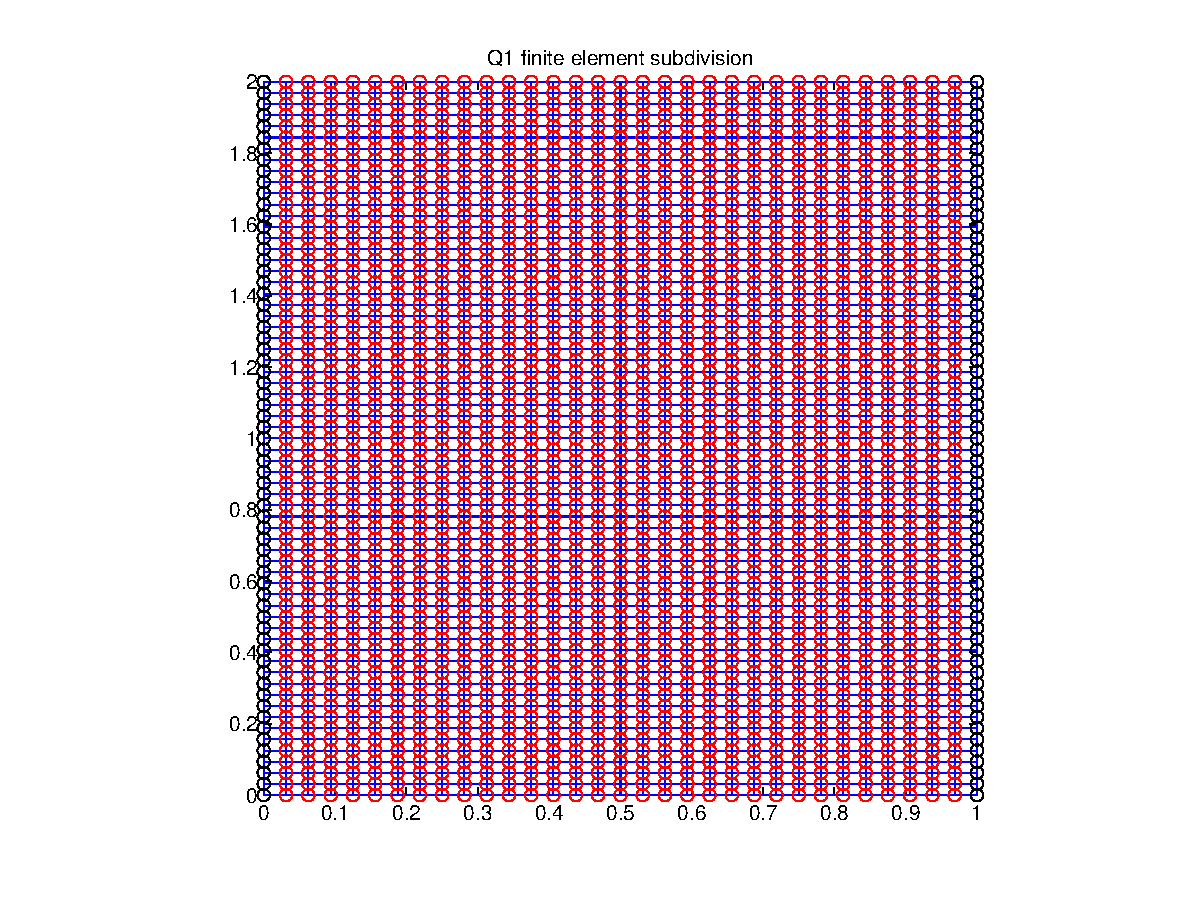
\includegraphics[width=4.1in]{untitled.eps}
\end{figure} 
\end{frame}

\section{建立矩阵-$Au=f$}

\begin{frame}
\begin{figure}[!ht]
\centering
\includegraphics[width=4.1in]{图1.PNG}
\end{figure} 
\end{frame}

%
\begin{frame}
\frametitle{建立矩阵-$Au=f$}
\begin{itemize}
\item 矩形元的所有点的局部-全局映射由下式给出
\begin{eqnarray*}
x(\xi,\eta)&=&x_1\chi_1(\xi,\eta)+x_2\chi_2(\xi,\eta)+x_3\chi_3(\xi,\eta)+x_4\chi_4(\xi,\eta)\\
y(\xi,\eta)&=&y_1\chi_1(\xi,\eta)+y_2\chi_2(\xi,\eta)+y_3\chi_3(\xi,\eta)+y_4\chi_4(\xi,\eta)
\end{eqnarray*}
\item $\chi_1(\xi,\eta),\chi_2(\xi,\eta),\chi_3(\xi,\eta),\chi_4(\xi,\eta)$是Q1基函数。
\item 
\newcommand{\ud}{\mathrm{d}}
\begin{displaymath}
a_{ij}^{(k)}=\int_{\Box\ast}\left\{\frac{\partial\psi_{\ast,i}}{\partial x}\frac{\partial\psi_{\ast,j}}{\partial x}+\frac{\partial\psi_{\ast,i}}{\partial y}\frac{\partial\psi_{\ast,j}}{\partial y}\right\}|J_k|\ud\xi \ud\eta
\end{displaymath}
\begin{displaymath}
f_i^{(k)}=\int_{\Box\ast}f\psi_{\ast,i}|J_k|\ud\xi \ud\eta
\end{displaymath}

\end{itemize}
\end{frame}

%
\begin{frame}
\frametitle{建立矩阵-$Au=f$}
\begin{itemize}
\item 使用高斯求积法来求解上述的定积分
\end{itemize}
\begin{displaymath}
\overline a_{ij}^{(k)}=\sum_{s=1}^m\sum_{t=1}^mw_{st}|J_k(\xi_s,\eta_t)|\left\{\frac{\partial\psi_{\ast,i}}{\partial x}\frac{\partial\psi_{\ast,j}}{\partial x}+\frac{\partial\psi_{\ast,i}}{\partial y}\frac{\partial\psi_{\ast,j}}{\partial y}\right\}\bigg{|}_{(\xi_s,\eta_t)}
\end{displaymath}
\begin{displaymath}
\overline f_i^{(k)}=\sum_{s=1}^m\sum_{t=1}^mw_{st}f(\xi_{s},\eta_t)\psi_{\ast,i}(\xi_{s},\eta_t)|J_k(\xi_{s},\eta_t)|
\end{displaymath}
\end{frame}

\section{求解方程}

%
\begin{frame}
\frametitle{求解方程-TR} 
\begin{itemize}
\item 使用稳定梯形法则
\begin{displaymath}
M\dot{u}+Au=f \qquad u(0)=u_0
\end{displaymath}
给出向量$u_n\approx u(t_n)$, $u_{n+1}\approx u(t_n+\triangle t_n)$,求解隐式系统
\begin{displaymath}
u_{n+1}=u_n+M^{-1}(f-\frac{1}{2}A(u_{n+1}+u_n))
\end{displaymath}
\end{itemize}
\end{frame}

\end{document}
